\documentclass{article}
\usepackage{iclr2027_conference,times}
\usepackage[T1]{fontenc}
\usepackage[utf8]{inputenc}
\usepackage{amsmath,amssymb,amsthm,booktabs,graphicx,microtype}
\usepackage{xcolor,url,hyperref}
\hypersetup{colorlinks=true,linkcolor=blue,citecolor=blue,urlcolor=blue}

% Single manuscript. All prose, notation, tables, and proofs are in this file.
% The official ICLR 2027 style is unmodified. Default: anonymous review format.
% SPECTRUM is the paper name for the repository's spectral_soft method.
\newcommand{\method}{\textsc{Spectrum}}
\newcommand{\R}{\mathbb{R}}
\newcommand{\E}{\mathbb{E}}
\newcommand{\I}{\mathbf{I}}
\newcommand{\D}{\mathcal{D}}
\newcommand{\Cbar}{\bar C}
\DeclareMathOperator{\diag}{diag}
\DeclareMathOperator{\tr}{tr}
\DeclareMathOperator*{\argmin}{arg\,min}
\newtheorem{proposition}{Proposition}

% Float separation. The template leaves these at the LaTeX article default of
% 12pt; 9pt is used so that the nine-page main-text limit is met without
% removing content. This adjusts spacing only -- no style or class file is
% modified, and no other dimension of the template is touched.
\setlength{\textfloatsep}{9pt plus 2pt minus 2pt}
\setlength{\intextsep}{9pt plus 2pt minus 2pt}
\setlength{\floatsep}{9pt plus 2pt minus 2pt}

\title{SPECTRUM: Soft Spectral Self-Distillation\\Preserves Correct-Code Diversity}
\author{Anonymous Authors}

\begin{document}
\maketitle

\begin{abstract}
Self-distillation from a model's own raw outputs is a cheap and widely used way to improve code models, and it is judged by correctness alone. Correctness, however, does not identify \emph{which} correct programs a model produces. Two models with identical pass@$k$ can expose completely different sets of correct implementations, and it is that set --- not the accuracy number --- that the next distillation round trains on. We measure the missing quantity over five self-distillation rounds of Qwen2.5-Coder-1.5B-Instruct on MBPP. Every arm we test loses correct-implementation coverage relative to the undistilled model while pass@1 rises, so the loss is invisible in the metric the field reports. The loss is not fixed: it is governed by the generation-time intervention. We introduce \method, which replaces the hard rank truncation of spectral self-distillation with a full-rank continuous proximal gain. A quadratic penalty yields a closed-form operator whose gains lie in $[1/(1+\tau),1]$, so no direction is zeroed at finite strength. After five rounds \method\ retains $89.9\%$ of the undistilled model's 64-sample coverage, where plain self-distillation retains $66.4\%$ and hard projection $65.5\%$, and it is the only arm whose pass@64 estimate exceeds the undistilled model's, significantly above both comparators ($+2.4$ pp over hard projection, $95\%$ CI $[0.6,4.4]$). It gives up $1.4$ pp of pass@1 against hard projection; we report that cost rather than hide it.
\end{abstract}

\section{Introduction}
\label{sec:intro}

Self-distillation from raw model outputs is one of the cheapest ways to improve a code model: sample completions, keep the ones that pass a test, train on them, repeat. The recipe is evaluated, almost universally, by a correctness number --- pass@1, or pass@$k$ at some budget. That number answers how \emph{often} the model succeeds. It does not answer \emph{which} correct programs it produces.

The distinction is not cosmetic, and it is not identified by any pass@$k$. Consider a task with $c$ distinct correct implementations. Let $a_\theta$ be the probability that a single sample is correct, and let $D_b(\theta)$ be the expected number of distinct correct implementations appearing in $b$ \emph{correct} draws. Two models can agree on $a_\theta$ --- and therefore on every pass@$k$, which is a functional of the correctness marginal alone --- while differing arbitrarily in $D_b$. Section~\ref{sec:problem} makes this precise. The consequence for self-distillation is direct: a round filters the corpus by correctness, so what the next student inherits is the \emph{conditional} distribution over correct implementations, and nothing in the loop measures it.

We measure it. Over five generate$\to$LoRA rounds of Qwen2.5-Coder-1.5B-Instruct on MBPP we track both the usual accuracy endpoints and correctness-matched implementation coverage, using AST fingerprints as an implementation-structure proxy. Two findings emerge, and they pull in opposite directions.

\emph{First, coverage erodes in every arm, and accuracy rises anyway.} Relative to the undistilled checkpoint, all three distillation arms end five rounds with less correct-implementation coverage --- the two comparators declining monotonically, \method\ flattening at round~5 --- while pass@1 rises monotonically in all three (Figure~\ref{fig:problem}). After five rounds the undistilled model's 64-sample coverage of $12.80$ AST classes per task falls to $8.51$ under plain self-distillation and $8.39$ under hard spectral projection --- a loss of roughly a third --- while pass@1 moves from $37.9\%$ to $41.4\%$ and $41.8\%$. The field's headline metric improves while the property it is blind to degrades.

\emph{Second, the loss is not a fixed cost of distillation; it is governed by the generation-time intervention.} The three arms share a pipeline and differ only in how the correctness-gradient spectrum is used to shape generation. Plain self-distillation loses $4.30$ coverage units of $12.80$; SPD-style hard rank truncation loses $4.41$; the arm we introduce loses $1.29$. Since hard projection is the one existing method that explicitly intervenes on this axis, the result is uncomfortable for it: intervening \emph{harder} on the spectrum made coverage worse, not better.

We introduce \method\ (Section~\ref{sec:method}). It keeps the pipeline of spectral self-distillation --- calibrate a second moment of correctness-gradient K/V directions, shape generation with it, train normally on everything generated --- and replaces the one discontinuous step. Where hard projection zeroes all but the top-$r$ eigendirections, \method\ solves a quadratic proximal problem whose closed-form solution has eigenvalues $1/[1+\tau(1-\mu_j)]$: a continuous ramp rather than a cutoff. Three properties follow at once. The gains live in $[1/(1+\tau),1]$, so \emph{no direction is ever zeroed} at finite strength and the operator is full rank. The operator is a bounded perturbation of the identity, $\|T-\I\|_2 \le \tau/(1+\tau) < 1$. And it is cheap: a single eigendecomposition folded temporarily into the generation weights and restored before ordinary LoRA training, so the student never inherits the transform.

Empirically, \method\ is the arm that keeps the most of what the undistilled model had. It retains $89.9\%$ of the base model's 64-sample coverage where plain self-distillation retains $66.4\%$ and hard projection $65.5\%$, and on the per-round tier the margin over hard projection compounds: the paired advantage on four-correct-draw coverage grows monotonically from $+0.066$ in round~1 to $+0.293$ in round~5, with every interval excluding zero (Figure~\ref{fig:compounding}). It also retains an accuracy advantage that the other arms do not: \method\ is the only arm whose pass@64 exceeds the undistilled model's, significantly above both comparators.

Against hard projection specifically, the accuracy ledger is mixed and we state it plainly. \method\ is $1.43$ pp \emph{lower} on pass@1 (95\% CI $[-1.89,-0.98]$) but $2.4$ pp \emph{higher} on pass@64 (95\% CI $[0.6,4.4]$). The declared noninferiority criterion for pass@1 against this comparator is not met. We do not reframe this as a trade-off or as noninferiority; it is a cost, and Section~\ref{sec:limits} lists it among the paper's limitations.

\paragraph{Contributions.} \textbf{(1)~A measurement argument.} Correctness and correctness-conditioned implementation coverage are different objectives, and no pass@$k$ identifies the second (Section~\ref{sec:problem}); current self-distillation work reports only the first. \textbf{(2)~An empirical finding.} Repeated self-distillation reduces correctness-matched implementation coverage below the undistilled model in every arm tested, and the existing hard-projection intervention reduces it most (Section~\ref{sec:results}). \textbf{(3)~A method.} A full-rank continuous spectral gain derived from correctness gradients, with a proximal interpretation, a closed form, a contraction bound, and exact temporary weight folding (Section~\ref{sec:method}, Proposition~\ref{prop:gain}). \textbf{(4)~A measured effect under a frozen protocol.} The continuous gain retains markedly more coverage than plain self-distillation and hard projection after five rounds, while beating both at pass@64 and trailing both at pass@1.

\begin{figure}[t]
  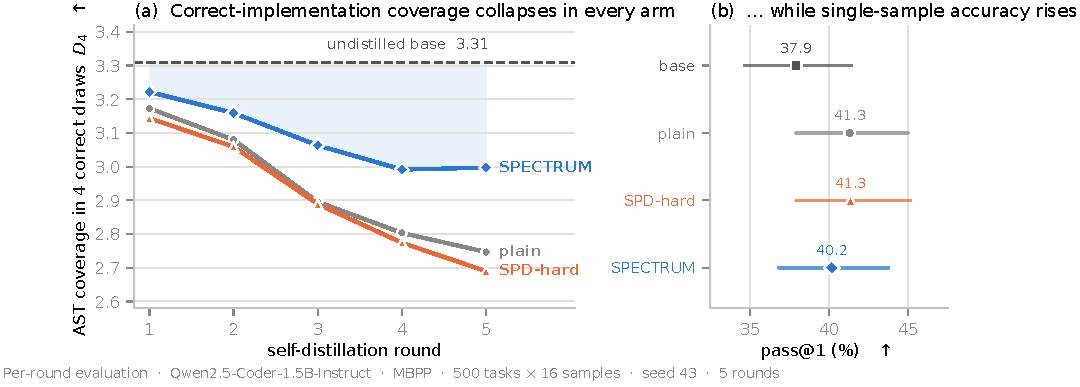
\includegraphics[width=\textwidth]{figures/fig1_problem.pdf}
  \caption{\small Self-distillation erodes correct-implementation coverage in every arm, while single-sample accuracy rises. Five generate$\to$LoRA rounds on MBPP (291 synthesis tasks, seed 43), evaluated on all 500 held-out test tasks with 16 samples each round. \textbf{(a)} Correct-implementation coverage $D_4$ --- the expected number of distinct AST implementation classes in four \emph{correct} draws --- falls below the undistilled level (dashed rule) in all three arms. The continuous-gain arm (\method) falls least; the other two fall about twice as far. \textbf{(b)} The same arms at round 5 are all \emph{more} accurate single-shot than the undistilled model, so the coverage loss is invisible in the metric the field reports. Intervals are $95\%$ task-bootstrap. Coverage uses only tasks with at least four correct samples in that arm (256--270 of 500) and accuracy uses all 500, so the two panels have different denominators. AST fingerprints proxy implementation structure, not audited algorithm identity.}
  \label{fig:problem}
\end{figure}

\section{Correctness does not identify implementation coverage}
\label{sec:problem}

Fix a task with a test suite. Write $\mathcal{P}$ for the set of programs that pass it, and partition $\mathcal{P}$ into equivalence classes by an implementation fingerprint $\phi$ --- here, a normalized AST skeleton with identifiers and literals abstracted away. Let $c = |\phi(\mathcal{P})|$ be the number of distinct correct implementation classes, and let $p_1,\dots,p_c$ be the class probabilities under the model's sampling distribution $\pi$ (with $\pi_0$ the mass on incorrect programs).

Pass@1 is $a = 1-\pi_0$. The expected number of distinct correct classes in $b$ correct draws is
\begin{equation}
\label{eq:db}
D_b \;=\; \sum_{j=1}^{c}\Bigl[1 - \frac{\binom{c-c_j}{b}}{\binom{c}{b}}\Bigr],
\qquad c_j = \lfloor c\,p_j \rfloor \ \text{or the finite-sample analogue},
\end{equation}
where $c_j$ counts the samples drawn from class $j$; we compute it directly by sampling without replacement from the observed class counts, so the definition is exact for the measured arm. Equation~\eqref{eq:db} is the correct-draw analogue of pass@$b$: it conditions on correctness and asks how much of the correct surface the $b$ surviving draws cover.

The two quantities are not reducible to one another. Pass@$k$ is a function of $a$ and the sample count; it is invariant under any reallocation of mass \emph{among} correct classes that preserves $a$. $D_b$ is not: it depends on the whole vector $(p_1,\dots,p_c)$. A model that emits one correct program with probability $a$ has $D_b\to 1$; a model that spreads the same mass uniformly over $c$ correct classes has $D_b \to \min(b,c)$. Both report the same pass@1 and the same pass@64.

This is why the metric matters for self-distillation and not merely for evaluation. A round samples from $\pi$, keeps what passes, and trains on the result, so what the student learns is the conditional distribution over correct programs --- precisely the object $D_b$ summarizes and no accuracy endpoint measures. A round can therefore raise pass@1 and reduce $D_b$ simultaneously, and the loop will not notice. Section~\ref{sec:results} shows that this is what happens.

\paragraph{A second endpoint, not a rescaling.} Coverage at a $k$-sample budget, $C_k$ --- the total number of distinct correct classes among $k$ samples, \emph{without} conditioning on success --- is a different endpoint from $D_b$: $C_k$ grows with $k$ and includes incorrect mass, while $D_b$ is fixed at $b$ correct draws. The two are reported side by side in our tables and must never share an axis.

\section{\method: a continuous gain on the correctness spectrum}
\label{sec:method}

\subsection{Protocol}
\label{sec:protocol}

A round $t$ starts from a native checkpoint $\theta_t$ and produces $\theta_{t+1}$ in three steps. (i) A reference-completion loss supplies gradients with respect to the outputs of the key and value linear layers at decoder layers $\lfloor L/2\rfloor$ and $L-1$, at \emph{every} nonpadding position including prompt positions. Masking the loss and selecting positions are different operations, and we do not conflate them. (ii) Those gradients define a second-moment matrix, from which an operator is built and folded temporarily into the generation weights. (iii) The folded model emits one raw completion per training prompt; every completion --- including wrong and empty ones --- enters the corpus. Ordinary LoRA is then initialized from the \emph{saved native} $\theta_t$ and trained on all nonpadding targets, and the result is merged into $\theta_{t+1}$. Evaluation always uses the merged native model with no transform applied. Figure~\ref{fig:method} shows the pipeline; the only step that differs between the arms we compare is (ii).

\begin{figure}[t]
  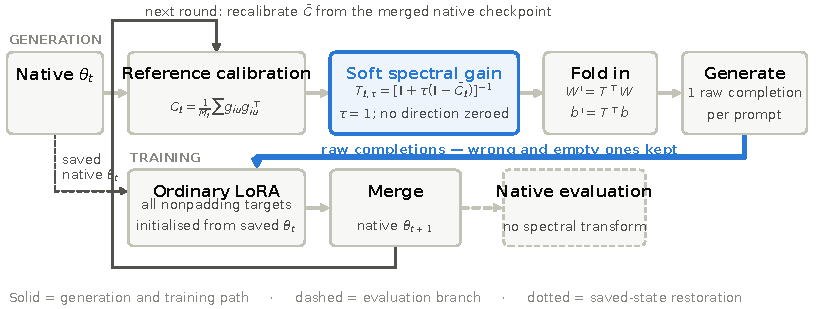
\includegraphics[width=\textwidth]{figures/fig2_method.pdf}
  \caption{\small \method\ changes the distribution the training data is drawn from, not the training objective. Reference-completion loss supplies gradients of the native K/V linear outputs at every nonpadding position; their normalized second moment defines a full-rank continuous gain $T_{\ell,\tau}$ folded \emph{temporarily} into the generation weights. Every raw completion enters the corpus, and LoRA then starts from the saved native $\theta_t$, so the student never inherits the transform. The merged native $\theta_{t+1}$ is evaluated without any transform and is what the next round recalibrates from. Solid arrows: generation and training path; dashed: evaluation; dotted: saved-state restoration.}
  \label{fig:method}
\end{figure}

\subsection{The correctness-gradient spectrum}
\label{sec:spectrum}

For a selected module $\ell$, let $g^{(\ell)}_{iu}\in\R^{d}$ be the gradient of the reference-completion loss with respect to the module's output activation at position $u$ of example $i$. Because the loss is masked, some positions contribute a zero gradient; $M_\ell$ counts \emph{all} included positions, zeros included, so the normalization is a true average rather than a mean over a gradient-dependent support. We form
\begin{equation}
\label{eq:C}
C_\ell \;=\; \frac{1}{M_\ell}\sum_{i,\,u\ \text{nonpad}} g^{(\ell)}_{iu}\, g^{(\ell)\top}_{iu},
\qquad
\Cbar_\ell \;=\; \frac{C_\ell}{\lambda_{\max}(C_\ell)},
\end{equation}
so that $\Cbar_\ell$ is symmetric positive semidefinite with spectrum in $[0,1]$. Write $\mu_1\ge\dots\ge\mu_d$ for its eigenvalues. A large $\mu_j$ means the reference solution's gradient has a strong, consistent component along direction $j$: the model is already being told, by a correct completion, to move in that direction. A small $\mu_j$ means the reference barely exercises it.

The design intent of spectral self-distillation is to down-weight the directions the reference does not exercise, biasing generation toward reference-like behavior. The existing implementation does this by projection: keep the top-$r$ eigendirections, discard the rest, so the gains are $1$ on $r$ directions and $0$ on $d-r$ of them. We keep the intent and remove the discontinuity.

\subsection{A continuous gain}
\label{sec:gain}

Rather than choose which directions to keep, we penalize the operator's deviation from the identity in proportion to how little the reference exercises each direction. Let $T\in\R^{d\times d}$ and minimize
\begin{equation}
\label{eq:prox}
f(T) \;=\; \tfrac12\|T-\I\|_F^2 \;+\; \tfrac{\tau}{2}\,\tr\!\bigl(T(\I-\Cbar_\ell)T^\top\bigr),
\qquad \tau>0 .
\end{equation}
The first term keeps the intervention small; the second is a quadratic penalty whose cost is large along directions with small $\mu_j$, since $\I-\Cbar_\ell$ has eigenvalues $1-\mu_j$ there. Because $\I-\Cbar_\ell$ is positive semidefinite, $f$ is strongly convex and the minimizer is unique.

\begin{proposition}
\label{prop:gain}
The minimizer of Eq.~\eqref{eq:prox} is
\begin{equation}
\label{eq:T}
T_{\ell,\tau} \;=\; \bigl[\I+\tau(\I-\Cbar_\ell)\bigr]^{-1},
\qquad\text{with eigenvalues}\qquad
s_\tau(\mu_j) \;=\; \frac{1}{1+\tau\,(1-\mu_j)} .
\end{equation}
Consequently: \emph{(i)} $s_\tau$ is continuous and strictly increasing on $[0,1]$, with $s_\tau(0)=1/(1+\tau)$ and $s_\tau(1)=1$, so the gains lie in $[1/(1+\tau),1]$ and \emph{no direction is zeroed at any finite $\tau$}; $T_{\ell,\tau}$ is full rank. \emph{(ii)} $T_{\ell,\tau}\to\I$ as $\tau\to0^{+}$ and the intervention increases monotonically in $\tau$. \emph{(iii)} $\|T_{\ell,\tau}-\I\|_2 = \tau/(1+\tau) < 1$, so the operator is a bounded perturbation of the identity for every $\tau$. \emph{(iv)} $T_{\ell,\tau}$ is symmetric, and its action on a vector costs one eigendecomposition of $\Cbar_\ell$ and a scaling of the coefficients.
\end{proposition}

\noindent A proof is in Appendix~\ref{app:proof}. The default is $\tau=1$, giving gains in $[\tfrac12,1]$: the least-exercised direction is halved rather than deleted.

Figure~\ref{fig:operator} contrasts the two profiles on shared axes. The hard projector is a step function --- gains of exactly $0$ below the cut, exactly $1$ above it --- and its discarded set is a hard decision made from a finite reference set, which will under-exercise directions a slightly different reference would have exercised. The continuous ramp makes the same ordering decision with a graded response, and Proposition~\ref{prop:gain}(iii) bounds how far it can move the policy at all. This is a design rationale, not a verified mechanism: the controls that would isolate which property produces the measured effect were implemented but not run (Section~\ref{sec:limits}).

\begin{figure}[t]
  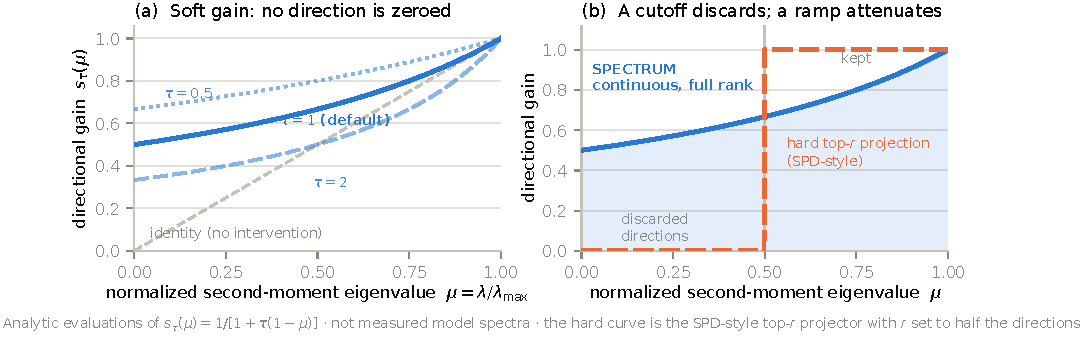
\includegraphics[width=\textwidth]{figures/fig3_operator.pdf}
  \caption{\small The soft gain and the contrast it replaces. Analytic evaluations of $s_\tau(\mu)=1/[1+\tau(1-\mu)]$, not measured model spectra. \textbf{(a)} For every finite $\tau$ the profile is bounded away from zero, so all directions survive; the floor $1/(1+\tau)$ moves with the strength dial. \textbf{(b)} On shared axes at $\tau=1$, the hard top-$r$ projector is a step: directions below the cut receive gain exactly $0$, and $r$ is half the directions, as in our reconstruction of the hard baseline.}
  \label{fig:operator}
\end{figure}

\subsection{Temporary folding}
\label{sec:folding}

The operator acts on the module output, so it can be pushed into the weights exactly: for a linear layer $y = Wx + b$ we set $W' = T^\top W$ and $b' = T^\top b$ in float32 and use the folded layer for generation only. Because the folded parameters are exact in exact arithmetic, the saved native values are restored before any training step, and LoRA is initialized from the restored $\theta_t$. The student therefore trains against a corpus drawn from a shaped distribution but never inherits the shaping; the next round recomputes $C_\ell$ from the merged native $\theta_{t+1}$, which is also the model that is evaluated.

\section{Experimental setup}
\label{sec:setup}

\paragraph{Model and data.} Qwen2.5-Coder-1.5B-Instruct \citep{hui2024qwen25coder} throughout. MBPP \citep{austin2021mbpp} is split into 291 synthesis tasks, from which the round's training prompts are drawn, and 500 held-out test tasks used only for evaluation. Evaluation executes candidate programs against the task tests locally; the official EvalPlus container was not used.

\paragraph{Rounds.} Five generate$\to$LoRA rounds, training seed 43, for each of three arms that differ \emph{only} in step (ii) of Section~\ref{sec:protocol}: \emph{plain} (no intervention), \emph{SPD-hard} (top-$r$ eigendirections retained, $r$ half the directions, reconstruction from the released method description), and \method\ at $\tau=1$. A fourth, \emph{SSD}-style arm with a temperature/top-$p$ generation recipe exists only in a separate single-round 64-task pilot (Appendix~\ref{app:pilot}); it is not part of the five-round comparison. The undistilled checkpoint is evaluated once and serves as a reference level, not as a fourth trajectory.

\paragraph{Two evaluation tiers, kept apart.} The \emph{per-round tier} evaluates every arm after every round on all 500 tasks with 16 samples per task; it is the only tier with per-round measurements, and Figures~\ref{fig:problem} and~\ref{fig:compounding} use it. The \emph{final tier} re-evaluates the undistilled checkpoint and the three round-5 checkpoints on all 500 tasks with 64 samples per task; it gives tighter estimates but exists only at round 5, and Tables~\ref{tab:main} and~\ref{tab:paired} and Figure~\ref{fig:effects} use it. The two tiers have different sample budgets and are never mixed within a claim. Throughout, pass@$k$ uses the unbiased finite-sample estimator, and $C_k$ is normalized coverage at a $k$-sample budget.

\paragraph{Statistics.} All intervals are $95\%$ task-bootstrap intervals over 2000 replicates. Comparisons are \emph{paired}: a task enters a covered comparison only if it supplies at least the required number of correct samples in \emph{both} arms, so the eligible set shrinks with $b$: on the 64-sample tier the $D_4$ comparisons run on 311--318 of 500 tasks, $D_8$ on 283--296, $D_{16}$ on 237--254 and $D_{64}$ on 18--30, while accuracy and $C_k$ comparisons use all 500. Intervals are pointwise; no multiplicity correction is applied across the many endpoints in Tables~\ref{tab:main} and~\ref{tab:paired}. Everything reported is one training seed; the five rounds are sequential, not independent replicates, so no seed-level uncertainty is available.

\section{Results}
\label{sec:results}

\begin{table}[t]
\caption{\small Final checkpoint, 64-sample tier. All 500 held-out MBPP tasks, 64 samples per task, seed 43. ``ret.'' is the fraction of the undistilled level retained. $C_k$ is correct-implementation coverage at a $k$-sample budget; $D_b$ is coverage in $b$ \emph{correct} draws (Eq.~\eqref{eq:db}) over tasks supplying at least $b$ correct samples, so the $D_b$ columns rest on 251--323 tasks and the $C_k$ and pass@$k$ columns on all 500. Best value in each column in \textbf{bold}, excluding the reference row.}
\label{tab:main}
\centering\small
\begin{tabular}{lrrrrrrrr}
\toprule
 & \multicolumn{2}{c}{accuracy} & \multicolumn{2}{c}{coverage ($C_k$)} & \multicolumn{3}{c}{correct-draw ($D_b$)} & \\
\cmidrule(lr){2-3}\cmidrule(lr){4-5}\cmidrule(lr){6-8}
Arm & pass@1 & pass@64 & $C_{8}$ & $C_{64}$ & $D_{4}$ & $D_{8}$ & $D_{16}$ & ret.\ ($D_{16}$) \\
\midrule
Undistilled & 37.94 & 72.00 & 2.267 & 12.802 & 3.358 & 5.987 & 10.423 & --- \\
\midrule
plain       & 41.45 & 70.40 & 1.923 & 8.506 & 2.856 & 4.690 & 7.324 & 70.3\% \\
SPD-hard    & \textbf{41.77} & 70.20 & 1.892 & 8.388 & 2.810 & 4.590 & 7.136 & 68.5\% \\
\method     & 40.33 & \textbf{72.60} & \textbf{2.161} & \textbf{11.510} & \textbf{3.143} & \textbf{5.451} & \textbf{9.091} & \textbf{87.2\%} \\
\bottomrule
\end{tabular}
\end{table}

\subsection{Every arm loses coverage; accuracy rises anyway}
\label{sec:erosion}

Figure~\ref{fig:problem}(a) traces four-correct-draw coverage across the five rounds. The undistilled checkpoint sits at $D_4 = 3.310$. Plain self-distillation falls monotonically to $2.747$; hard projection falls monotonically to $2.690$; \method\ falls to $2.997$. Two features of the panel carry the finding: the decline is monotone in the two comparator arms --- it is not noise around a flat line --- and the panel's companion (Figure~\ref{fig:problem}b) shows that the same arms are all \emph{more} accurate single-shot at round 5 than the undistilled model.

The final tier makes the magnitude concrete (Table~\ref{tab:main}). At 64 samples per task the undistilled model covers $12.80$ distinct correct AST classes per task. Plain self-distillation covers $8.51$ and hard projection $8.39$, retentions of $66.4\%$ and $65.5\%$. The ordering is not an artifact of the 64-sample budget: it reappears at small budgets and widens in the correct-draw endpoints, where the three arms retain $91.1\%$, $78.3\%$ and $76.7\%$ at $D_8$ and $87.2\%$, $70.3\%$ and $68.5\%$ at $D_{16}$.

\begin{figure}[t]
  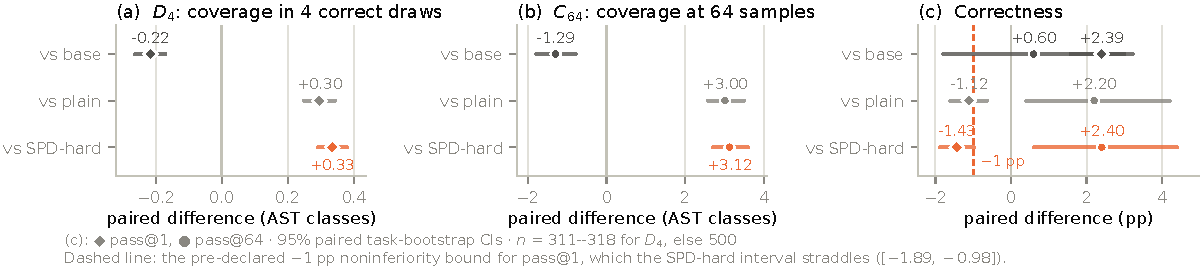
\includegraphics[width=\textwidth]{figures/fig4_effects.pdf}
  \caption{\small Paired effects at the round-5 checkpoint, 64-sample tier (500 MBPP tasks $\times$ 64 samples, seed 43). Positive means \method\ is higher. $D_4$ and $C_{64}$ are different endpoints, so panels (a) and (b) carry separate axes rather than sharing one. \textbf{(a)} $D_4$: \method\ is below the undistilled model but far above both distilled comparators, by $+0.33$ AST classes against hard projection. \textbf{(b)} $C_{64}$: the same ordering, by $+3.12$. \textbf{(c)} Correctness: \method\ is above the undistilled model on pass@1 and below both comparators, but the sign reverses at pass@64, where it is above all three. The dashed line is the pre-declared $-1$ pp noninferiority bound for pass@1; the \method$-$SPD-hard interval, $[-1.89,-0.98]$, straddles it, so the criterion---that the lower bound be no lower than $-1$ pp---is not met. Intervals are $95\%$ task-bootstrap, paired on shared eligible tasks, pointwise (no multiplicity correction); $n=311$--$318$ paired tasks for $D_4$ and $500$ for all other endpoints.}
  \label{fig:effects}
\end{figure}

\subsection{The intervention decides how much is lost}
\label{sec:intervention}

The three arms share a pipeline, a data split, a seed, and a training procedure. They differ in one step. Yet the coverage they \emph{lose} differs by a factor of three: $4.41$ units under hard projection, $4.30$ under plain self-distillation, and $1.29$ under \method\ (Table~\ref{tab:main}, $C_{64}$). Because hard projection is the one prior method that intervenes deliberately on this axis, this ordering is a finding about it rather than about self-distillation in general.

The paired comparisons in Table~\ref{tab:paired} and Figure~\ref{fig:effects}(a,b) confirm that the separation is not a level effect. Against hard projection, \method\ gains $+0.334$ AST classes on $D_4$ (95\% CI $[0.290,0.379]$) and $+3.12$ on $C_{64}$ (95\% CI $[2.69,3.60]$). Against plain self-distillation the gains are $+0.295$ and $+3.00$. Against the undistilled model, \method\ is \emph{below} on coverage on both endpoints --- the erosion is real and \method\ does not undo it, it only slows it.

\begin{table}[t]
\caption{\small Paired differences, \method\ minus reference, round-5 checkpoint. Accuracy in percentage points, coverage in AST classes per task; positive means \method\ is higher. Intervals are $95\%$ task-bootstrap, paired on shared eligible tasks, pointwise. The pre-declared pass@1 noninferiority criterion (interval lower bound $\ge -1$ pp) is stated in Appendix~\ref{app:protocol}.}
\label{tab:paired}
\centering\small
\begin{tabular}{lrrrr}
\toprule
Reference & $\Delta$pass@1 (pp) & $\Delta$pass@64 (pp) & $\Delta C_{64}$ & $\Delta D_4$ \\
\midrule
Undistilled & $+2.39\ [1.58,\,3.22]$ & $+0.6\ [-1.8,\,3.0]$ & $-1.29\ [-1.79,\,-0.78]$ & $-0.216\ [-0.263,\,-0.171]$ \\
plain       & $-1.12\ [-1.61,\,-0.63]$ & $+2.2\ [0.4,\,4.2]$ & $+3.00\ [2.57,\,3.49]$ & $+0.295\ [0.249,\,0.343]$ \\
SPD-hard    & $-1.43\ [-1.89,\,-0.98]$ & $+2.4\ [0.6,\,4.4]$ & $+3.12\ [2.69,\,3.60]$ & $+0.334\ [0.290,\,0.379]$ \\
\bottomrule
\end{tabular}
\end{table}

\subsection{The advantage compounds over rounds}
\label{sec:compound}

The separation is not a fixed offset acquired early and then carried. Figure~\ref{fig:compounding}(a) plots the paired difference in $D_4$ between \method\ and hard projection at each round: $+0.066$, $+0.127$, $+0.162$, $+0.229$, $+0.293$. Every interval excludes zero, and the sequence is monotone. Whatever the continuous gain is doing, it is not a one-time correction; the two arms diverge progressively as the loop runs.

Panel (b) places the same rounds against the undistilled level. Plain self-distillation and hard projection descend in a near-parallel band, reaching $-0.57$ and $-0.63$ AST classes by round 5. \method\ descends to $-0.32$ and flattens between rounds 4 and 5 ($2.9914 \to 2.9971$). We report the flattening but do not build on it: it is a single-seed difference of $0.006$ with overlapping intervals, and a plateau would need more rounds to establish.

\begin{figure}[t]
  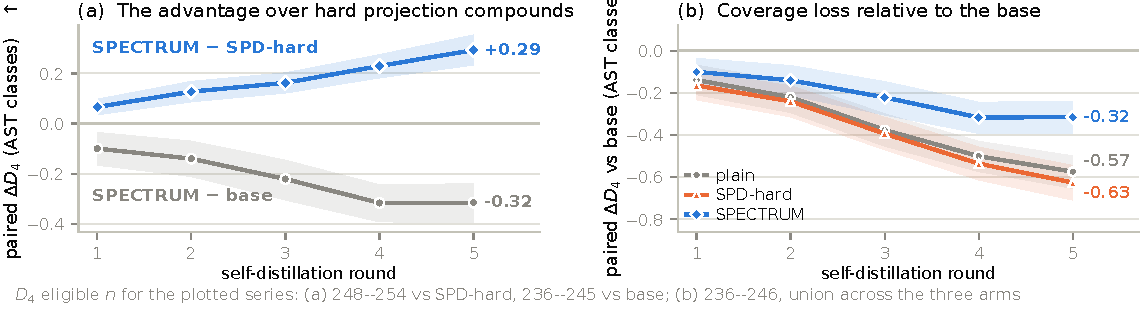
\includegraphics[width=\textwidth]{figures/fig5_compounding.pdf}
  \caption{\small The coverage advantage compounds, and the loss relative to the undistilled model saturates. Per-round tier (500 tasks $\times$ 16 samples, seed 43); shaded bands and annotated endpoints are $95\%$ task-bootstrap intervals, paired on shared eligible tasks ($D_4$ eligible $n$: $248$--$254$ against SPD-hard, $236$--$245$ for \method\ against the undistilled model, $236$--$246$ across all three arms of panel (b)). \textbf{(a)} The advantage over hard projection grows monotonically from $+0.066$ in round 1 to $+0.293$ in round 5, every interval excluding zero; the deficit against the undistilled model deepens and then holds. \textbf{(b)} The same rounds as a paired difference from the undistilled level: the two comparator arms descend nearly in parallel to about $-0.6$ AST classes by round 5, while \method's deficit stops near $-0.32$.}
  \label{fig:compounding}
\end{figure}

\subsection{Accuracy: better at large budgets, worse at one draw}
\label{sec:accuracy}

On the final tier \method\ is third of four on pass@1 ($40.33\%$ against $41.77\%$ for hard projection and $41.45\%$ for plain) but first on pass@$64$ ($72.60\%$ against $70.20\%$ and $70.40\%$) and it is the only arm whose pass@$64$ exceeds the undistilled model's $72.00\%$. The paired differences make the pattern sharp (Table~\ref{tab:paired}, Figure~\ref{fig:effects}c): against hard projection, $-1.43$ pp on pass@1 (95\% CI $[-1.89,-0.98]$) and $+2.4$ pp on pass@$64$ (95\% CI $[0.6,4.4]$); against plain, $-1.12$ pp and $+2.2$ pp; against the undistilled model, $+2.39$ pp on pass@1 and an inconclusive $+0.6$ pp on pass@$64$.

This signature --- lower single-draw accuracy, higher large-budget success --- is what a method that widens the output distribution should produce, and it is consistent with the coverage results rather than in tension with them. It is nevertheless a real cost at the budget most papers report: \textbf{the pre-declared noninferiority criterion for pass@1 against hard projection is not met.} The criterion required the interval's lower bound to be no lower than $-1$ pp; it comes in at $-1.89$ pp. We do not describe the accuracy change as a trade-off --- only one direction of any such trade-off was measured against the same comparator under the same conditions, and the other direction is the coverage gain, a different endpoint --- nor as noninferior, because the interval excludes zero on the unfavourable side. The full criterion is restated in Appendix~\ref{app:protocol}.

One qualification belongs here. The pass@1 gap against hard projection is close to the margin: its verdict flips across rounds in the per-round tier, where the paired difference is $-0.09$, $-0.84$, $-0.35$, $-1.31$ and $-1.18$ pp at rounds 1--5 and the noninferiority criterion is met at rounds 1 and 3 but not at 2, 4 and 5. The point estimate is stably negative from round 2 onward; its position relative to a $-1$ pp bound is not.

\subsection{Heterogeneity across fingerprint families}
\label{sec:hetero}

All coverage endpoints above use a normalized AST skeleton. We also computed a coarser control-flow proxy fingerprint that merges implementations differing only in expression-level detail; these are per-round-tier measurements, as the final tier carries no control-flow block. The effect is family-dependent, and we report the case where it disappears: against hard projection at round 5 the control-flow difference is $+0.042$, CI $[-0.011,0.095]$, which includes zero, even though the AST endpoint on the same tasks and pairing is decisively positive. Against the undistilled model on the same tier the control-flow deficit is still present ($-0.131$, CI $[-0.199,-0.063]$). The gain therefore concentrates in implementation-structure distinctions that a coarse control-flow abstraction discards; we report both families rather than the favourable one.

\section{Related work}
\label{sec:related}

\paragraph{Self-distillation and synthetic data.} Training on a model's own filtered outputs is a standard recipe, from self-instruct-style bootstrapping \citep{wang2023selfinstruct} to recent raw-output self-distillation for code \citep{zhang2026ssd}; it has also been analyzed as function-space regularization, in the supervised setting \citep{mobahi2020selfdistillation} and through conceptors \citep{postmus2024conceptors}. This line evaluates with correctness. We ask what it does to the conditional distribution over correct outputs, and find a systematic cost the correctness metric does not register.

\paragraph{Spectrum-based selection.} The closest antecedent is spectral self-distillation \citep{hao2026spd}, which builds a second moment of correctness-gradient directions and retains its leading eigendirections. Section~\ref{sec:intervention} reproduces that construction faithfully and finds it the weakest arm on coverage; Section~\ref{sec:gain} replaces the truncation with a proximal ramp. Reward-shaped selection \citep{hu2026rewardingrare} intervenes on the same pipeline at a different point, reweighting samples by difficulty rather than shaping generation. Both redistribute mass over generations, and the question we raise applies to them equally.

\paragraph{Model collapse and diversity evaluation.} Recursive training on generated data is known to lose distributional tails \citep{shumailov2024collapse}, and accumulating real alongside synthetic data mitigates it \citep{gerstgrasser2024accumulating}; those analyses are over the full data distribution, whereas ours is over the much smaller object a correctness filter leaves behind. For code, pass@$k$ \citep{chen2021humaneval} and EvalPlus \citep{liu2023evalplus} measure success at a budget, and AST-based deduplication is standard for \emph{cleaning} training data; we use the same fingerprints as a measurement, on the correct-draw endpoint $D_b$ rather than the coverage-at-a-budget endpoint $C_k$, because only the former answers the question a distillation loop needs answered. Sea-of-identities-style analysis \citep{qiu2024sea} likewise argues that aggregate correctness hides structure, in decoding rather than distillation.

\paragraph{Adaptation and proximal operators.} Our intervention is applied to generation weights only and removed before LoRA \citep{hu2022lora} training begins, so it is neither an adapter nor a fine-tuning method. The closed form in Proposition~\ref{prop:gain} is the standard proximal solution for a quadratic penalty \citep{parikh2014proximal}, applied here to a gradient second moment rather than to parameters.

\section{Limitations}
\label{sec:limits}

\paragraph{The accuracy cost is real.} \method\ is $1.12$--$1.43$ pp below both distilled comparators on pass@1 and fails the pre-declared noninferiority criterion against both. It beats both at pass@$64$ and beats the undistilled model on pass@1, but a practitioner whose budget is one sample per task should prefer plain self-distillation under our measurements.

\paragraph{Diversity claims are structural.} AST fingerprints proxy implementation structure, not semantic algorithm identity. The blinded algorithm annotation that would support an algorithm-level claim was designed and never executed; every ``coverage'' statement in this paper is about AST classes.

\paragraph{The mechanism is not isolated.} The controls that would attribute the effect to a specific property of the operator --- matched blends, random-eigenvector substitution, isotropic alternatives --- are implemented but unrun. Proposition~\ref{prop:gain} characterizes the operator; it does not show that its continuity is what produces the measured coverage retention.

\paragraph{Single seed, single model, single benchmark.} Everything reported is training seed 43 on Qwen2.5-Coder-1.5B-Instruct on MBPP. Rounds are sequential and not independent replicates. No second benchmark and no transfer result (HumanEval+/EvalPlus) were run, and the 3B configuration exists but is unrun. The paired bootstrap cannot be recomputed from the released bundle, which retains hashes rather than per-task records.

\paragraph{Execution environment.} Candidate programs were executed locally rather than in the official EvalPlus container.

\section{Conclusion}
\label{sec:conclusion}

Self-distillation is justified by accuracy and evaluated by accuracy, and the accuracy number is blind to the set of correct implementations the loop teaches the next student. Over five rounds that set measurably contracts in every arm we tested, including the prior method that intervenes on this axis deliberately. The choice of intervention is not a detail: a continuous, full-rank proximal gain loses roughly a third as much of the undistilled model's correct-implementation coverage as plain self-distillation or hard projection, and its advantage compounds across rounds, at the price of about a point of single-sample accuracy against those comparators. The practical implication is narrow and actionable: report a correctness-conditioned coverage endpoint next to pass@$k$, and treat the strength of a spectral intervention as a dial rather than a cutoff.

\subsubsection*{AI use statement}
An AI coding assistant helped organize the experimental records, generate the figures from the stored result files, and edit the prose. All experimental results came from the authors' code; every numerical value was transcribed from the stored result files and checked against them. No results, citations, or statistics were generated by the assistant.

\bibliography{references}
\bibliographystyle{iclr2027_conference}

\appendix
\renewcommand{\thesection}{\Alph{section}}

\section{Protocol and the pre-declared success criterion}
\label{app:protocol}

The confirmatory protocol was frozen before the five-round run. It declares a round-5 result a success if \emph{both} conditions hold against \emph{each} comparator:
\begin{enumerate}\itemsep2pt
\item the paired difference in four-correct-draw AST coverage, $D_4$, is positive, i.e.\ its $95\%$ task-bootstrap interval excludes zero and lies above it; and
\item the paired pass@1 difference is noninferior at a margin of $1$ percentage point, i.e.\ the interval's lower bound is $\ge -0.01$.
\end{enumerate}
Measured against hard projection at round 5 on the 16-sample tier, condition~1 holds ($+0.293$, CI $[0.233,0.353]$) and condition~2 fails ($-0.0118$, CI $[-0.0190,-0.0048]$). Against the undistilled model condition~1 cannot hold by construction --- the paired $D_4$ difference is $-0.315\ [-0.394,-0.240]$, the erosion the criterion exists to detect --- while condition~2 does hold ($+0.0225$, CI $[0.0120,0.0335]$). Against plain the 16-sample tier supplies no paired comparison; the 64-sample tier does, and condition~1 holds there ($+0.295$) while condition~2 fails ($-1.12$~pp). The declared criterion is therefore met against neither distilled comparator. The same two conditions on the 64-sample tier give the rows of Table~\ref{tab:paired}, where condition~1 holds against both distilled arms and condition~2 fails against both. We report the criterion in its original form rather than restating it after the fact.

\section{Full paired comparisons}
\label{app:full}

Table~\ref{tab:full} lists every paired comparison on the 64-sample tier, including endpoints not discussed in the main text. Entries are point estimates with $95\%$ task-bootstrap intervals; $n$ is the number of paired eligible tasks, which differs across endpoints because $D_b$ requires $b$ correct samples in both arms.

\begin{table}[h]
\caption{\small All paired differences, \method\ minus reference, 64-sample tier, round 5. Accuracy entries are percentage points; coverage entries are AST classes per task. Intervals are pointwise $95\%$ task-bootstrap intervals with no multiplicity correction. $D_{64}$ is included for completeness but rests on only 18--30 paired eligible tasks and should not be read as an estimate of the same quality as the others.}
\label{tab:full}
\centering\scriptsize
\begin{tabular}{llrrrrr}
\toprule
Endpoint & vs & $\Delta$ & \multicolumn{2}{c}{95\% CI} & $n$ \\
\midrule
pass@1   & undistilled & $+2.39$ & $+1.58$ & $+3.22$ & 500 \\
pass@4   & undistilled & $+1.14$ & $+0.07$ & $+2.17$ & 500 \\
pass@8   & undistilled & $+0.80$ & $-0.32$ & $+2.02$ & 500 \\
pass@16  & undistilled & $+0.53$ & $-0.87$ & $+1.97$ & 500 \\
pass@64  & undistilled & $+0.60$ & $-1.80$ & $+3.00$ & 500 \\
$C_{4}$  & undistilled & $-0.023$ & $-0.057$ & $+0.012$ & 500 \\
$C_{8}$  & undistilled & $-0.106$ & $-0.172$ & $-0.036$ & 500 \\
$C_{16}$ & undistilled & $-0.281$ & $-0.410$ & $-0.147$ & 500 \\
$C_{64}$ & undistilled & $-1.292$ & $-1.786$ & $-0.780$ & 500 \\
$D_{4}$  & undistilled & $-0.216$ & $-0.263$ & $-0.171$ & 311 \\
$D_{8}$  & undistilled & $-0.566$ & $-0.671$ & $-0.455$ & 283 \\
$D_{16}$ & undistilled & $-1.342$ & $-1.588$ & $-1.091$ & 237 \\
$D_{64}$ & undistilled & $-5.222$ & $-7.451$ & $-3.000$ & 18 \\
\midrule
pass@1   & plain & $-1.12$ & $-1.61$ & $-0.63$ & 500 \\
pass@4   & plain & $-0.33$ & $-0.93$ & $+0.30$ & 500 \\
pass@8   & plain & $+0.04$ & $-0.66$ & $+0.73$ & 500 \\
pass@16  & plain & $+0.59$ & $-0.24$ & $+1.39$ & 500 \\
pass@64  & plain & $+2.20$ & $+0.40$ & $+4.20$ & 500 \\
$C_{4}$  & plain & $+0.078$ & $+0.052$ & $+0.103$ & 500 \\
$C_{8}$  & plain & $+0.238$ & $+0.183$ & $+0.296$ & 500 \\
$C_{16}$ & plain & $+0.599$ & $+0.487$ & $+0.723$ & 500 \\
$C_{64}$ & plain & $+3.004$ & $+2.568$ & $+3.494$ & 500 \\
$D_{4}$  & plain & $+0.295$ & $+0.249$ & $+0.343$ & 316 \\
$D_{8}$  & plain & $+0.780$ & $+0.665$ & $+0.889$ & 296 \\
$D_{16}$ & plain & $+1.816$ & $+1.582$ & $+2.055$ & 254 \\
$D_{64}$ & plain & $+5.276$ & $+3.545$ & $+7.150$ & 29 \\
\midrule
pass@1   & SPD-hard & $-1.43$ & $-1.89$ & $-0.98$ & 500 \\
pass@4   & SPD-hard & $-0.38$ & $-0.94$ & $+0.18$ & 500 \\
pass@8   & SPD-hard & $+0.02$ & $-0.64$ & $+0.63$ & 500 \\
pass@16  & SPD-hard & $+0.58$ & $-0.18$ & $+1.35$ & 500 \\
pass@64  & SPD-hard & $+2.40$ & $+0.60$ & $+4.40$ & 500 \\
$C_{4}$  & SPD-hard & $+0.091$ & $+0.066$ & $+0.116$ & 500 \\
$C_{8}$  & SPD-hard & $+0.269$ & $+0.215$ & $+0.324$ & 500 \\
$C_{16}$ & SPD-hard & $+0.655$ & $+0.544$ & $+0.770$ & 500 \\
$C_{64}$ & SPD-hard & $+3.122$ & $+2.686$ & $+3.596$ & 500 \\
$D_{4}$  & SPD-hard & $+0.334$ & $+0.290$ & $+0.379$ & 318 \\
$D_{8}$  & SPD-hard & $+0.875$ & $+0.773$ & $+0.979$ & 295 \\
$D_{16}$ & SPD-hard & $+1.998$ & $+1.792$ & $+2.218$ & 254 \\
$D_{64}$ & SPD-hard & $+5.533$ & $+3.928$ & $+7.207$ & 30 \\
\bottomrule
\end{tabular}
\end{table}

\section{Per-round ledger}
\label{app:perround}

Table~\ref{tab:perround} gives the per-round tier in full: each arm's level at each round, and the paired difference of \method\ against each reference. Table~\ref{tab:perrounddelta} gives the accuracy side of the same rounds.

\begin{table}[h]
\caption{\small Per-round tier (500 tasks $\times$ 16 samples, seed 43). The undistilled row carries $95\%$ task-bootstrap intervals; arm rows are point values. Deltas are paired on shared eligible tasks. Coverage unit: AST classes per task.}
\label{tab:perround}
\centering\scriptsize
\begin{tabular}{llrrrr}
\toprule
Arm & round & pass@1 (\%) & $D_4$ & eligible $n$ \\
\midrule
undistilled & --- & $37.92\ [34.69,41.40]$ & $3.310\ [3.221,3.400]$ & 262 \\
\midrule
plain & 1 & $38.42$ & $3.173$ & 261 \\
plain & 2 & $39.15$ & $3.080$ & 269 \\
plain & 3 & $39.65$ & $2.895$ & 257 \\
plain & 4 & $40.79$ & $2.803$ & 270 \\
plain & 5 & $41.30$ & $2.747$ & 268 \\
\midrule
SPD-hard & 1 & $37.92$ & $3.144$ & 257 \\
SPD-hard & 2 & $39.20$ & $3.059$ & 267 \\
SPD-hard & 3 & $39.40$ & $2.889$ & 256 \\
SPD-hard & 4 & $41.09$ & $2.774$ & 266 \\
SPD-hard & 5 & $41.35$ & $2.690$ & 262 \\
\midrule
\method & 1 & $37.84$ & $3.222$ & 261 \\
\method & 2 & $38.36$ & $3.159$ & 259 \\
\method & 3 & $39.05$ & $3.063$ & 262 \\
\method & 4 & $39.78$ & $2.991$ & 263 \\
\method & 5 & $40.18$ & $2.997$ & 263 \\
\bottomrule
\end{tabular}
\end{table}

\begin{table}[h]
\caption{\small Paired per-round differences, \method\ minus reference, per-round tier. Positive means \method\ is higher. ``NI'' is the pre-declared $-1$ pp pass@1 criterion of Appendix~\ref{app:protocol}.}
\label{tab:perrounddelta}
\centering\scriptsize
\begin{tabular}{rlrrrr}
\toprule
vs & round & $\Delta$pass@1 (pp) & NI & $\Delta D_4$ & $n$ \\
\midrule
undistilled & 1 & $-0.09$ & \checkmark & $-0.100\ [-0.166,-0.035]$ & 242 \\
undistilled & 2 & $+0.44$ & \checkmark & $-0.140\ [-0.211,-0.070]$ & 236 \\
undistilled & 3 & $+1.12$ & \checkmark & $-0.221\ [-0.305,-0.146]$ & 244 \\
undistilled & 4 & $+1.85$ & \checkmark & $-0.316\ [-0.392,-0.244]$ & 242 \\
undistilled & 5 & $+2.25$ & \checkmark & $-0.315\ [-0.394,-0.240]$ & 245 \\
\midrule
SPD-hard & 1 & $-0.09\ [-0.56,+0.42]$ & \checkmark & $+0.066\ [+0.035,+0.097]$ & 250 \\
SPD-hard & 2 & $-0.84\ [-1.42,-0.24]$ & $\times$ & $+0.127\ [+0.086,+0.168]$ & 254 \\
SPD-hard & 3 & $-0.35\ [-0.91,+0.31]$ & \checkmark & $+0.162\ [+0.122,+0.202]$ & 248 \\
SPD-hard & 4 & $-1.31\ [-1.98,-0.66]$ & $\times$ & $+0.229\ [+0.182,+0.275]$ & 249 \\
SPD-hard & 5 & $-1.18\ [-1.90,-0.48]$ & $\times$ & $+0.293\ [+0.233,+0.353]$ & 251 \\
\bottomrule
\end{tabular}
\end{table}

\section{Single-round pilot, including an SSD-style arm}
\label{app:pilot}

The five-round comparison above does not contain an SSD-style arm, because the SSD decoding recipe was only run in an earlier exploratory pilot. That pilot used 64 held-out MBPP tasks, 64 samples per task, seed 42, one distillation round, and a first-fence extraction rule; its numbers are therefore not comparable to the main run's and are reported here only because it is the sole place an SSD-style control appears.

In the pilot, four arms land within $0.24$ pp of each other on pass@1 (plain $36.82\%$, SSD $36.89\%$, SPD-hard $36.87\%$, \method\ $36.65\%$) and within $0.03$ AST classes on $D_4$ ($3.393$, $3.391$, $3.409$, $3.422$). Against the SSD-style control, \method's paired final-checkpoint differences are $+0.0312$ AST classes on $D_4$ (95\% CI $[0.0095,0.0550]$), $+0.0083$ on exact-program unique fraction ($[0.0009,0.0171]$), $-0.244$ pp on pass@1 ($[-0.854,+0.342]$) and $+3.125$ pp on pass@64 ($[0,+7.813]$). The pilot's own analysis concludes that these are exploratory and not evidence of distinct semantic algorithms, and we concur: the effect size there is an order of magnitude smaller than the five-round AST-coverage effect measured above, which is consistent with the main finding being a property of \emph{repeated} rounds rather than of a single one.

\section{Proof of Proposition~\ref{prop:gain}}
\label{app:proof}

Write $S = \I-\Cbar_\ell$, which is symmetric with eigenvalues $1-\mu_j \in [0,1]$. The objective in Eq.~\eqref{eq:prox} is
$f(T) = \tfrac12\tr\bigl((T-\I)(T-\I)^\top\bigr) + \tfrac{\tau}{2}\tr\bigl(T S T^\top\bigr)$.
Since $S\succeq 0$ and $\tau>0$, the second term is convex and the first is strongly convex, so $f$ has a unique minimizer. Its gradient is
\[
\nabla f(T) = (T-\I) + \tau T S ,
\]
using $\nabla_T \tr(TS T^\top) = 2TS$ for symmetric $S$. Setting the gradient to zero gives $T(\I+\tau S) = \I$, i.e.\
\[
T_{\ell,\tau} = (\I+\tau S)^{-1} = \bigl[\I+\tau(\I-\Cbar_\ell)\bigr]^{-1}.
\]
$S$ is symmetric and thus orthogonally diagonalizable, $S = Q\Lambda Q^\top$ with $\Lambda=\diag(1-\mu_j)$. Hence $T_{\ell,\tau} = Q\,\diag\!\bigl(1/(1+\tau(1-\mu_j))\bigr)Q^\top$, which is symmetric with the stated eigenvalues $s_\tau(\mu_j)$.

For (i): $s_\tau$ is a M\"obius function of $\mu_j$, strictly increasing on $[0,1]$ with $s_\tau(0)=1/(1+\tau)$ and $s_\tau(1)=1$; every eigenvalue is therefore strictly positive, so $T_{\ell,\tau}$ is full rank and no direction is annihilated. For (ii): $s_\tau(\mu)\to1$ pointwise as $\tau\to0^+$, and $\partial s_\tau/\partial\tau = -(1-\mu)/(1+\tau(1-\mu))^2 \le 0$ with equality only at $\mu=1$, so the attenuation increases monotonically in $\tau$ in every direction except the leading one. For (iii): the eigenvalues of $T_{\ell,\tau}-\I$ are $\frac{\mu_j-1}{1+\tau(1-\mu_j)}\tau$, whose magnitudes are maximized at $\mu_j=0$, giving $\|T_{\ell,\tau}-\I\|_2 = \tau/(1+\tau) < 1$ for all $\tau<\infty$, with $\tau/(1+\tau)\to1$ only as $\tau\to\infty$. For (iv): one eigendecomposition of $\Cbar_\ell$ suffices; applying $T_{\ell,\tau}$ to a vector is a change of basis, a diagonal scaling, and a change back. $\square$

\paragraph{Relation to hard projection.} The hard baseline replaces $\Lambda$ by the indicator of the top-$r$ eigenvalues, i.e.\ $s^{\text{hard}}(\mu_j) = \mathbb{1}[\mu_j \ge \mu_{(r)}]$. This is the $\tau\to\infty$ limit of a rescaled ramp composed with a threshold, and it is not attained by $T_{\ell,\tau}$ at any finite $\tau$: for every finite $\tau$ the operator has full rank, whereas the hard projector has rank $r$. The two therefore differ in kind, not only in degree, and the difference is exactly the nullspace.

\section{Mechanism controls: design and status}
\label{app:controls}

The paper's central empirical claim is comparative, not mechanistic: among interventions on the same pipeline, the continuous gain retains the most coverage. Isolating \emph{which} property of the operator produces that retention requires controls that were implemented but not run before this submission. We list them so that the gap is explicit rather than implied.
\begin{itemize}\itemsep2pt
\item \textbf{Matched blend.} Mix the hard projection with the identity at a strength chosen so that its mean gain equals the continuous ramp's, testing whether the effect follows from continuity or merely from a weaker average attenuation.
\item \textbf{Random-eigenvector substitution.} Replace $\Cbar_\ell$'s eigenvectors with a random orthonormal basis while keeping the eigenvalue profile, testing whether the correctness-gradient directions carry any of the effect at all.
\item \textbf{Isotropic alternative.} A single scalar gain at matched average strength, testing whether the spectrum's shape matters beyond its mean.
\end{itemize}
None of these has a result to report. Proposition~\ref{prop:gain} characterizes the operator, and Section~\ref{sec:intervention} measures the outcome, but the causal path between them is open.

\end{document}
